\documentclass{beamer}

\usepackage{amsmath,amssymb}
\usepackage{tikz}
\usetikzlibrary{arrows,decorations,decorations.markings}

%
% Custom theme
%
\usetheme{AAUsimple}

%
% Custom operator declarations
%
\DeclareMathOperator{\ZZ}{\mathbb{Z}}
\DeclareMathOperator{\CC}{\mathbb{C}}
\DeclareMathOperator{\hh}{\mathfrak{h}}
\DeclareMathOperator{\re}{\text{Re}}
\DeclareMathOperator{\im}{\text{Im}}
\newcommand{\thetachar}[2] {\theta {\scriptsize \begin{bmatrix}#1\\#2\end{bmatrix}}}
\newcommand{\thetacharsm}[2] {\theta \left[ \begin{smallmatrix} #1
      \\ #2 \end{smallmatrix} \right]}

%%%%%%%%%%%%%%%%%%%%%%%%%%%%%%%%%%%%%%%%%%%%%%%%%%%%%%%%%%%%%%%%%%%%%%%%%%%%%%%
\title{Computational Geometry of Complex Algebraic Curves}
\subtitle{General Examination}
\author{
  Chris Swierczewski\\
  {\tt cswiercz@uw.edu}
}
\institute{
  Department of Applied Mathematics\\
  University of Washington\\
  Seattle, Washington
}
\pgfdeclareimage[height=1.5cm]{titlepagelogo}{AAUgraphics/aau_logo_new_circle}
\titlegraphic{
  \pgfuseimage{titlepagelogo}
}

\AtBeginSection[]{\begin{frame}\frametitle{Goal of This Talk}\tableofcontents[currentsection,subsectionstyle=show/show/shaded]\end{frame}}
%%%%%%%%%%%%%%%%%%%%%%%%%%%%%%%%%%%%%%%%%%%%%%%%%%%%%%%%%%%%%%%%%%%%%%%%%%%%%%%



%%%%%%%%%%%%%%%%%%%%%%%%%%%%%%%%%%%%%%%%%%%%%%%%%%%%%%%%%%%%%%%%%%%%%%%%%%%%%%%
\begin{document}
%%%%%%%%%%%%%%%%%%%%%%%%%%%%%%%%%%%%%%%%%%%%%%%%%%%%%%%%%%%%%%%%%%%%%%%%%%%%%%%



\begin{frame}[plain,noframenumbering]
  \titlepage
\end{frame}



%%%%%%%%%%%%%%%%%%%%%%%%%%%%%%%%%%%%%%%%%%%%%%%%%%%%%%%%%%%%%%%%%%%%%%%%%%%%%%%
%\section*{Introduction}
%%%%%%%%%%%%%%%%%%%%%%%%%%%%%%%%%%%%%%%%%%%%%%%%%%%%%%%%%%%%%%%%%%%%%%%%%%%%%%%

%------------------------------------------------------------------------------
%\subsection*{Shallow Water Waves}
%------------------------------------------------------------------------------



\begin{frame}{The Kadomtsev--Petviashvili Equation}{}
  \vspace{10pt}
  $u(x,y,t) = $ surface height of a 2d periodic shallow water wave.
  \[
  \tfrac{3}{4} u_{yy} = \frac{\partial}{\partial x} \left(
  u_t - \tfrac{1}{4} \left(6uu_x + u_{xxx}\right) \right)
  \]

  \begin{figure}
    \centering
    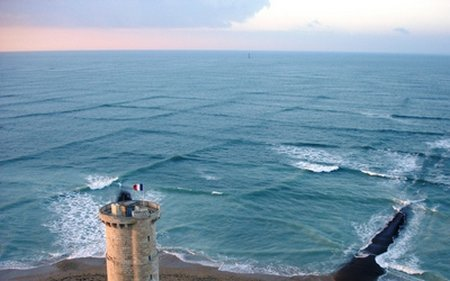
\includegraphics[height=0.4\textheight]{images/livekp.jpg}
    \caption{KP waves off the coast of \^{I}le de R\'{e}, France.}
  \end{figure}
\end{frame}



\begin{frame}{Theta Function Solutions}{}
  KP admits a (large) family of solutions of the form
  \[
  u(x,y,t) = 2 \partial_x^2 \log
  \theta(Ux + Vy + Wt + z_0, \Omega),
  \]
  where, for any $g \in \ZZ_+$,
  \begin{itemize}
    \item $U,V,W,z_0 \in \CC^g$,
    \item $\Omega \in \CC^{g \times g}$,
    \item $\theta : \CC^g \times \CC^{g \times g} \to \CC$
      is the {\it``Riemann theta function''}.
  \end{itemize}

  \vspace{16pt}

  Theta function solutions are \underline{dense} in the space of
  periodic solutions to KP. (Abelian functions.)
\end{frame}



\begin{frame}{The Riemann Theta Function}
  The Riemann theta function $\theta:\CC^g \times \CC^{g \times g} \to
  \CC$
  \begin{align*}
  \theta(z,\Omega)
  &=
  \sum_{n \in \ZZ^g}
  e^{
    2 \pi i
    \left( \tfrac{1}{2} n \cdot \Omega n + n \cdot z \right)
  } \\
  \thetachar{\alpha}{\beta}(z,\Omega)
  &=
  e^{2 \pi i \left( \tfrac{1}{2} \alpha \cdot \Omega \alpha + \alpha
    \cdot (z + \beta) \right)}
  \theta(z + \Omega \alpha + \beta, \Omega)
  \end{align*}

  \begin{block}{Convergence}
    $\im(\Omega)$ must be positive definite. Additionally, we only
    consider symmetric $\Omega$. So called space of ``Riemann
    matrices'': $\hh_g$.
  \end{block}
  \[
    \theta:\CC^g \times \hh_g \to \CC
  \]
\end{frame}



\begin{frame}{\phantom{Demo}}{}
  \begin{center}
    {\huge \it Demo}

    \vspace{1cm}

    Riemann theta functions.
  \end{center}
\end{frame}



%------------------------------------------------------------------------------
%\subsection*{Connection to Algebraic Geometry}
%------------------------------------------------------------------------------



\begin{frame}{Connection to Algebraic Geometry}{}
  \[
    u(x,y,t) = 2 \partial_x^2 \log
    \theta(Ux + Vy + Wt + z_0, \Omega)
  \]
  The constants $U,V,W,z_0,\Omega$ are not arbitrary. They come from a
  {\it complex algebraic curve}: given a polynomial $f \in
  \CC[\lambda,\mu]$
  \[
      f(\lambda,\mu) =
      \alpha_n(\lambda)\mu^n +
      \alpha_{n-1}(\lambda)\mu^{n-1} +
      \cdots +
      \alpha_0(\lambda)
  \]
  the curve $C$ is (basically) the set
  \[
  C = \left\{ (\lambda,\mu) \in \CC^2 \, : \, f(\lambda,\mu) = 0 \right\}.
  \]
\end{frame}



\begin{frame}{\tt abelfunctions}{}
  \setbeamercolor{block body}{use={block title},bg=block title.fg}
  \begin{block}{}
  \begin{figure}[t]
    \centering
    
\includegraphics[width=0.8\textwidth]{./images/abelfunctions.png}
  \end{figure}
  \end{block}

  \vspace{16pt}

  A Python library for computing with complex algebraic curves and
  Abelian functions.
  \begin{center}
    {\tt https://github.com/cswiercz/abelfunctions}

    {\tt https://www.cswiercz.info/abelfunctions}

  \end{center}
\end{frame}



\begin{frame}{Goal of This Talk}{}
  \tableofcontents
\end{frame}



%%%%%%%%%%%%%%%%%%%%%%%%%%%%%%%%%%%%%%%%%%%%%%%%%%%%%%%%%%%%%%%%%%%%%%%%%%%%%%%
\section{Algebraic Curves and Riemann Surfaces}
%%%%%%%%%%%%%%%%%%%%%%%%%%%%%%%%%%%%%%%%%%%%%%%%%%%%%%%%%%%%%%%%%%%%%%%%%%%%%%%

%------------------------------------------------------------------------------
\subsection{Introduction}
%------------------------------------------------------------------------------



\begin{frame}{Plane Algebraic Curves}{}
  Non-singular, irreducible polynomial $f \in \CC[x,y]$.
  \[
      C = \left\{ (x,y) \in \CC^2 \, : \, f(x,y) = 0 \right\}
      \cup
      \{\text{points at infinity}\}
  \]
  \begin{itemize}
    \item Non-singularity: $\nabla f \big|_C$ is nowhere zero.
    \item Points at infinity: (made explicit using projective curves /
      homogenization.)
    \item $y$-coverings: let $x$ vary over $\CC^*$. What are all
      possible $y$-roots?
  \end{itemize}
\end{frame}



\begin{frame}{Riemann Surfaces}{}
  \begin{center}
    {\it Every non-singular complex plane algebraic curve is a compact
      Riemann surface and vice versa.}
  \end{center}
  Riemann Surfaces
  \begin{itemize}
    \item\alt<1>{Connected, 1-dimensional complex manifold.}{{\it Every
        neighborhood of $P \in C$ looks like $U \subset
        \mathbb{C}$.} ($P$ is called a {\it ``place''}.)}
    \item<3-> Homeomorphic to a donut with $g$ holes.
      \begin{itemize}
        \item $g$ = {\it ``genus''}
      \end{itemize}
    \item<3-> Curve with singularities: {\it ``desingularize''} using
      blow-ups / Puiseux series.
      \begin{itemize}
        \item Places represented by these Puiseux series.
        \item Otherwise, $P = (\alpha, \beta)$.
      \end{itemize}
  \end{itemize}
\end{frame}



\begin{frame}{\phantom{Demo}}{}
  \begin{center}
    {\huge \it Demo}

    \vspace{1cm}

    Curves and singularities.
  \end{center}
\end{frame}



%------------------------------------------------------------------------------
\subsection{Geometry: Basis of Cycles}
%------------------------------------------------------------------------------



\begin{frame}{Geometry of Riemann Surfaces}{}
  \begin{figure}
  \centering
  \begin{tikzpicture}[scale=0.9]
    \colorlet{darkgreen}{green!50!gray}
    \colorlet{lightgray}{white!80!black}
    \colorlet{darkblue}{blue!50!gray}

    %% % Bezier Control Points
    %% \filldraw [gray] (-6,0) circle (2pt)
    %%                  (-6,1.5) circle (2pt)
    %%                  (-5,2.5) circle (2pt)
    %%                  (-3.5,2.5) circle (2pt)
    %%                  (-2,2.5) circle (2pt)
    %%                  (-1,1.5) circle (2pt)
    %%                  (0,1.5) circle (2pt);

    \uncover<1->{

    % the reference volume
    \draw[lightgray, thick]         (0,-1.5) arc (270:90:0.4cm and 1.5cm);
    \draw[lightgray, thick, dashed] (0,1.5)  arc (90:-90:0.4cm and 1.5cm);

    \begin{scope}[very thick]
    % Quadrant II of Torus
    % (other draw statements are flips / rotations)
    \draw (-6,0) ..
          controls (-6,1.5) and (-5,2.5) ..
          (-3.5,2.5) ..
          controls (-2,2.5) and (-1,1.5) ..
          (0,1.5);
    \draw[xscale=-1] (-6,0) ..
          controls (-6,1.5) and (-5,2.5) ..
          (-3.5,2.5) ..
          controls (-2,2.5) and (-1,1.5) ..
          (0,1.5);
    \draw[rotate=180] (-6,0) ..
          controls (-6,1.5) and (-5,2.5) ..
          (-3.5,2.5) ..
          controls (-2,2.5) and (-1,1.5) ..
          (0,1.5);
    \draw[yscale=-1] (-6,0) ..
          controls (-6,1.5) and (-5,2.5) ..
          (-3.5,2.5) ..
          controls (-2,2.5) and (-1,1.5) ..
          (0,1.5);

    % The Holes
    % (one hole at center shifted to outsides)
    \draw[xshift=-3.2cm] (-0.8,0) ..
          controls (-0.5,0.5) and (0.5,0.5) ..
          (0.8,0);
    \draw[yscale=-1,xshift=-3.2cm] (-1,-0.2) ..
          controls (-0.5,0.5) and (0.5,0.5) ..
          (1,-0.2);

    \draw[xshift=3.2cm] (-0.8,0) ..
          controls (-0.5,0.5) and (0.5,0.5) ..
          (0.8,0);
    \draw[yscale=-1,xshift=3.2cm] (-1,-0.2) ..
          controls (-0.5,0.5) and (0.5,0.5) ..
          (1,-0.2);
    }

    \uncover<1>{
    \draw (0,-3) node {$ \subset \CC^2$};
    }

    % a-cycles
    \uncover<2->{
    \draw[xshift=-3.2cm, darkblue, decoration={markings,
              mark=at position 0.25 with {\arrow[very thick]{latex}}},
          postaction={decorate}]
         (0,0) ellipse (2cm and 1.3cm);
    \draw[xshift=3.2cm, darkblue, decoration={markings,
              mark=at position 0.25 with {\arrow[very thick]{latex}}},
          postaction={decorate}]
         (0,0) ellipse (2cm and 1.3cm);

    % b-cycles
    \draw[xshift=-3.2cm, yshift=-2.47cm,
          darkgreen, decoration={markings,
              mark=at position 0.25 with {\arrow[very thick]{latex}}},
          postaction={decorate}]
         (0,0) arc (270:90:0.4cm and 1.07cm);
    \draw[xshift=-3.2cm, yshift=-0.33cm, dashed, darkgreen]
         (0,0) arc (90:-90:0.4cm and 1.07cm);
    \draw[xshift=3.2cm, yshift=-2.47cm,
          darkgreen, decoration={markings,
              mark=at position 0.25 with {\arrow[very thick]{latex}}},
          postaction={decorate}]
         (0,0) arc (270:90:0.4cm and 1.07cm);
    \draw[xshift=3.2cm, yshift=-0.33cm, dashed, darkgreen]
         (0,0) arc (90:-90:0.4cm and 1.07cm);

    % cycle labels
    \draw (-4,1.7)  node {$a_1$};
    \draw (4,1.7)   node {$a_2$};
    \draw (-3.2,-3) node {$b_1$};
    \draw (3.2,-3)  node {$b_2$};
    }

    \uncover<3>{
    % cycle intersection properties
    \draw (0,-3)   node {$a_i \circ a_j = 0$};
    \draw (0,-3.5) node {$b_i \circ b_j = 0$};
    \draw (0.1,-4) node {$a_i \circ b_j = \delta_{ij}$};
    }

    \uncover<4>{
    % homology
    \draw (0,-4) node
          {$H_1(C,\mathbb{Z}) = \text{span}\{a_1,\ldots,a_g,b_1,\ldots,b_g\}$};
    }
   \end{scope}
  \end{tikzpicture}
  \end{figure}
\end{frame}



\begin{frame}{\phantom{Demo}}{}
  \begin{center}
    {\huge \it Demo}

    \vspace{1cm}

    Basis of cycles.
  \end{center}
\end{frame}



%------------------------------------------------------------------------------
\subsection{Algebra: Holomorphic 1-forms}
%------------------------------------------------------------------------------



\begin{frame}{Integration on $\CC^*$}{}
  {\it What do we integrate on $\CC^*$?} Not functions
  \[
      \omega(z) : \CC^* \to \CC^*
  \]
  but {\it 1-forms}
  \[
      \omega = \omega(z)dz, \quad \omega(z) \text{ meromorphic}
  \]
  on paths $\gamma : [0,1] \to \CC^*, \gamma(t) = z(t)$.
  \[
      \int_\gamma \omega =
      \int_0^1 \omega \big( z(t) \big) dt
  \]
\end{frame}



\begin{frame}{Integration on $C : f(x,y) = 0$}{}
  {\it What do we integrate on $C$?} Not functions
  \[
      \omega(x,y) : \CC^* \times \CC^* \to C
  \]
  but {\it 1-forms}
  \[
      \omega = \omega(x,y)dx, \quad \omega(x,y) \text{ meromorphic}
  \]
  on paths $\gamma : [0,1] \to C, \gamma(t) = \big(x(t),y(t)\big)$.
  \[
      \int_\gamma \omega =
      \int_0^1 \omega \big( x(t), y(t) \big) x'(t) dt
  \]
\end{frame}



\begin{frame}{Holomorphic Differentials}{}
  \begin{block}{}
    The set of all {\it holomorphic} 1-forms on a genus $g$ Riemann
    surface $C$ forms a vector space over $\CC$
    \[
        H^1(C,\CC).
    \]
  \end{block}

  \begin{gather*}
      \dim_{\CC} H^1(C,\CC) = g \\
      \vspace{20pt} \\
      H^1(C,\CC) = \text{span} \left\{ \omega_1, \ldots, \omega_g \right\}
  \end{gather*}

  \begin{block}{}
    {\it Aside: why are there no holomorphic differentials on all of
      $\CC^*$?}
  \end{block}
\end{frame}



\begin{frame}{\phantom{Demo}}{}
  \begin{center}
    {\huge \it Demo}

    \vspace{1cm}

    Basis of 1-forms.
  \end{center}
\end{frame}



%------------------------------------------------------------------------------
\subsection{Period Matrices and the Abel Map}
%------------------------------------------------------------------------------



\begin{frame}{Period Matrices...}{}
  Matrices $A,B \in \CC^{g \times g}$:
  \[
      A_{ij} = \int_{a_j} \omega_i, \quad B_{ij} = \int_{b_j} \omega_i
  \]
  {\it ``Period matrix''} $\tau = [A \; B] \in \CC^{g \times 2g}$. \\
  \vspace{16pt}
  Possible to choose $\omega_i$'s such that
  \[
      \int_{a_j} \omega_i = \delta_{ij}.
  \]
  Period matrix:
  \[
      \tau = [I_{g \times g} \; \Omega].
  \]
\end{frame}



\begin{frame}{...and Riemann matrices}{}
  \begin{block}{Amazing Fact}
    $\Omega$ is a Riemann matrix.
  \end{block}
  \begin{block}{Schottky Problem}
    A Riemann matrix $\Omega$ comes from a period matrix \underline{if
      and only if}
    \[
        u(x,y,t) = 2 \partial_x^2 \log
        \theta(Ux + Vy + Wt + z_0, \Omega)
    \]
    satisfies the KP equation.
  \end{block}
  {\it \tiny (Some in the alg. geom. community don't like this proof.)}
\end{frame}



\begin{frame}{\phantom{Demo}}{}
  \begin{center}
    {\huge \it Demo}

    \vspace{1cm}

    Period / Riemann matrices.
  \end{center}
\end{frame}



%%%%%%%%%%%%%%%%%%%%%%%%%%%%%%%%%%%%%%%%%%%%%%%%%%%%%%%%%%%%%%%%%%%%%%%%%%%%%%%
\section{Goals and Applications}
%%%%%%%%%%%%%%%%%%%%%%%%%%%%%%%%%%%%%%%%%%%%%%%%%%%%%%%%%%%%%%%%%%%%%%%%%%%%%%%

%------------------------------------------------------------------------------
\subsection{Periodic Solutions to Integrable PDEs}
%------------------------------------------------------------------------------



\begin{frame}{Return to KP}{}
What do we need to constuct periodic solutions to KP?
\begin{gather*}
  u(x,y,t) = 2 \partial_x^2 \log \theta(Ux + Vy + Wt + z_0, \Omega) \\
  \uparrow \\
  C: f(\lambda,\mu) = 0, \quad \{n_i,P_i\} \in C \\
  \uncover<2->{
  \uparrow \\
  u(0,0,0), u'(0,0,0), \ldots, u^{(g-1)}(0,0,0)
  }
\end{gather*}
\uncover<2->{
{\bf Goal:} Develop black box algorithm for solving the I.V.P.
}
\end{frame}



\begin{frame}{Generalize Using Lax Pairs}{}
  Lax pair formulation:
  \[
      u_t = F(u,u_x,\ldots) \quad \leadsto \quad
      \begin{array}{c}
          X_t - T_x = [T,X], \\
          X = X(u,\lambda), T = T(u,\lambda)
      \end{array}
  \]
  Given Lax pair and $g$ initial data we can generate genus $g$ solution
  formula for any integrable equation. \\

  \vspace{16pt}

  {\bf Goal:} Develop black box algorithm for solving the I.V.P. for any
  given integrable PDE. (Given a Lax pair.)
\end{frame}



%------------------------------------------------------------------------------
\subsection{Linear Matrix Representations}
%------------------------------------------------------------------------------



\begin{frame}{Linear Matrix Representations}{}
  Every homogenous polynomial $F = F(x,y,z)$ can be written as
  \[
      F(x,y,z) = \det(Ax + By + Cz), \quad A,B,C \text{ symmetric}.
  \]
  Applications:
  \begin{itemize}
    \item formulation of problems in control theory,
    \item if $A,B,C \geq 0$, polynomial inequalities solvable by
      positive (semi) definite programming,
    \item study of two-dimensional {\it spectrahedra}: regions in
      $\mathbb{R}^2$ bounded by {\it Helton--Vinnikov curves}.
  \end{itemize}
\end{frame}



\begin{frame}{Computing $A,B,C$}{}
  Combinatorial Approach (Palumann, Sturmfels, Vinzant)
  \[
      O \left( 2^{d-2 \choose 2} \right)
      \text{ compute time}
  \]
  Helton--Vinnikov Theta Function Approach
  \[
      O \left( g^2 \right) \approx O \left( d^4 \right)
      \text{ compute time}
  \]
  Uses Abel map, theta with characteristic, and the {\it Schotty--Klein
    prime form}. \\

  \vspace{16pt}

  {\bf Goal:} Develop high-performance (high-accuracy) algorithms for
  computing LMRs.
\end{frame}


\begin{frame}{Schottky--Klein Prime Form}{}
  Riemann Surface ($g>0$) analogue of $f(z) = (z-\alpha)$.
  \begin{gather*}
      E : C \times C \to \mathbb{C}, \\
      E(P,Q) = \frac{
        \thetachar{\alpha}{\beta}
        \big(
        A(Q) - A(P)
        \big)
        }
      {
        \sqrt{\zeta(P)} \sqrt{\zeta(Q)}
      },
      \quad \zeta(P) = \nabla \thetachar{\alpha}{\beta}
      \big( 0, \Omega \big) \cdot (\omega_1, \ldots, \omega_g)
  \end{gather*}
  Modulo some universal covering space argument...
  \[
      E(P,Q) = 0 \quad \Leftrightarrow \quad P=Q.
  \]

  {\bf Goal:} Develop high-performance algorithms for computing prime
  forms and rational functions on Riemann surfaces.
\end{frame}


%------------------------------------------------------------------------------
\subsection{The Constructive Schottky Problem (*)}
%------------------------------------------------------------------------------



\begin{frame}{Schottky Problem}{}
  All period matrices give a Riemann matrix, but not vice versa.
  \begin{itemize}
    \item $\dim_{\CC} \{ \text{period matrices} \} = 3g-3$
    \item $\dim_{\CC} \mathfrak{h}_g = g(g+1)/2$
  \end{itemize}

  \vspace{16pt}

  \begin{block}{The Constuctive Schottky Problem}
    Given a Riemann matrix $\Omega$ can we produce a curve $C : f(x,y) =
    0$ with $\Omega$ as its period matrix?
  \end{block}

  \vspace{16pt}

  {\bf Goal (Long Term):} Compute this $f$.
\end{frame}


\begin{frame}[plain,noframenumbering]
  \finalpage{
    {\huge Thank you!} \\

    \vspace{20pt}

    {\tt \scriptsize https://github.com/cswiercz/abelfunctions}
    {\tt \scriptsize https://www.cswiercz.info/abelfunctions}
    {\tt \scriptsize https://github.com/cswiercz/general-exam}
  }
\end{frame}

\end{document}
